\documentclass[a4paper]{article}

\usepackage[utf8]{inputenc}
\usepackage[T1]{fontenc}
\usepackage{textcomp}
\usepackage[english]{babel}
\usepackage{amsmath, amssymb}


%figure support
\usepackage{import}
\usepackage{xifthen}
\pdfminorversion=7
\usepackage{pdfpages}
\usepackage{transparent}
\newcommand{\incfig}[1]{%
	\def\svgwidth{\columnwidth}
	\import{./figures/}{#1.pdf_tex}
}
\graphicspath{ {./figures/} }
\pdfsuppresswarningpagegroup=1

\begin{document}
	\title{EEL4768.04 Homework 7 Due 12/1/19}
	\author{Brandon Thompson 5517}
	\maketitle

	\begin{enumerate}
		\item Consider two interrupts $A$ and $B$. $A$ has higher priority than $B$. Interrupt
			Service Routine for $A$ is $ISR_{A}$ and Interrupt Service Routine for $B$ is
			$ISR_{B}$.\\
			How does the processor handle the interrupts when:
			\begin{enumerate}
				\item $A$ and $B$ both interrupt the processor at the same time.\\
					The processor will execute $ISR_A$ first because it has a
					higher priority, then it will execute $ISR_B$ and continue
					where the program left off.
				\item $A$ occurs first but before $ISR_{A}$ can be completed $B$
					interrupts the processor.\\
					The processor will finish executing $ISR_A$ because it has a
					higher priority, then it will execute $ISR_B$.
					
				\item $B$ occurs first but before $ISR_B$ can be completed $A$ interrupts
					the processor.\\
					The processor will save the state of $ISR_B$ and execute $ISR_A$ 
                                        then continue executing $ISR_B$.

			\end{enumerate}
		\item Use MIPS memory-mapped I/O to interact with a user. Each time the user presses a
			button, a pattern of your choice displays on five light-emitting diodes (LEDs).
			Suppose the input button is mapped to address \verb|0xFFFFFF10| and the LEDs
			are mapped to address \verb|0xFFFFFF14|. When the button is pushed, its
			output is 1; otherwise it is 0.\\
			Draw a schematic for this memory-mapped I/O system.
			\begin{figure}[ht!]
				\centering
				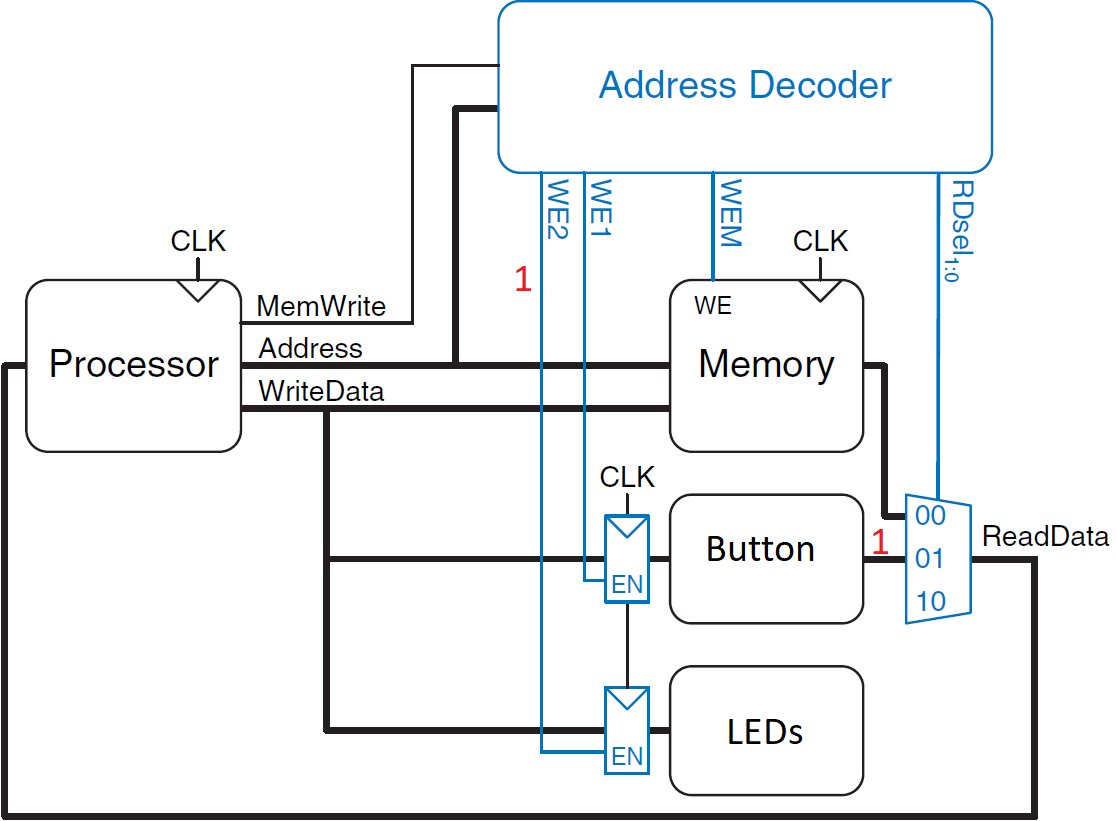
\includegraphics[width=\textwidth]{mem_map_io2}
				\caption{Button and LED memory-mapped I/O.}
				\label{fig:mem_map_io2}
			\end{figure}
	\end{enumerate}
\end{document}
